\documentclass{article}

\usepackage{fancyhdr}
\usepackage{extramarks}
\usepackage{amsmath}
\usepackage{amsthm}
\usepackage{amsfonts}
\usepackage{tikz}
\usepackage[plain]{algorithm}
\usepackage{algpseudocode}

\usetikzlibrary{automata,positioning}

%
% Basic Document Settings
%

\topmargin=-0.45in
\evensidemargin=0in
\oddsidemargin=0in
\textwidth=6.5in
\textheight=9.0in
\headsep=0.25in

\linespread{2.0}

\pagestyle{fancy}
\lhead{\hmwkAuthorName}
\chead{\hmwkClass\ (\hmwkClassInstructor\ \hmwkClassTime)}
\rhead{\firstxmark}
\lfoot{\lastxmark}
\cfoot{\thepage}

\renewcommand\headrulewidth{0.4pt}
\renewcommand\footrulewidth{0.4pt}

\setlength\parindent{0pt}

%
% Create Problem Sections
%

\newcommand{\enterProblemHeader}[1]{
    \nobreak\extramarks{}{Problem \arabic{#1} continued on next page\ldots}\nobreak{}
    \nobreak\extramarks{Problem \arabic{#1} (continued)}{Problem \arabic{#1} continued on next page\ldots}\nobreak{}
}

\newcommand{\exitProblemHeader}[1]{
    \nobreak\extramarks{Problem \arabic{#1} (continued)}{Problem \arabic{#1} continued on next page\ldots}\nobreak{}
    \stepcounter{#1}
    \nobreak\extramarks{Problem \arabic{#1}}{}\nobreak{}
}

\setcounter{secnumdepth}{0}
\newcounter{partCounter}
\newcounter{homeworkProblemCounter}
\setcounter{homeworkProblemCounter}{1}
\nobreak\extramarks{Problem \arabic{homeworkProblemCounter}}{}\nobreak{}

%
% Homework Problem Environment
%
% This environment takes an optional argument. When given, it will adjust the
% problem counter. This is useful for when the problems given for your
% assignment aren't sequential. See the last 3 problems of this template for an
% example.
%
\newenvironment{homeworkProblem}[1][-1]{
    \ifnum#1>0
        \setcounter{homeworkProblemCounter}{#1}
    \fi
    \section{Problem \arabic{homeworkProblemCounter}}
    \setcounter{partCounter}{1}
    \enterProblemHeader{homeworkProblemCounter}
}{
    \exitProblemHeader{homeworkProblemCounter}
}

%
% Homework Details
%   - Title
%   - Due date
%   - Class
%   - Section/Time
%   - Instructor
%   - Author
%

\newcommand{\hmwkTitle}{Homework\ \#7}
\newcommand{\hmwkDueDate}{October 26th, 2015}
\newcommand{\hmwkClass}{Differential Equation}
\newcommand{\hmwkClassTime}{Section 061}
\newcommand{\hmwkClassInstructor}{Professor Heather Lee}
\newcommand{\hmwkAuthorName}{Yao Xiao}

%
% Title Page
%

\title{
    \vspace{2in}
    \textmd{\textbf{\hmwkClass:\ \hmwkTitle}}\\
    \normalsize\vspace{0.1in}\small{Due\ on\ \hmwkDueDate\ at 3:10pm}\\
    \vspace{0.1in}\large{\textit{\hmwkClassInstructor\ \hmwkClassTime}}
    \vspace{3in}
}

\author{\textbf{\hmwkAuthorName}}
\date{}

\renewcommand{\part}[1]{\textbf{\large Part \Alph{partCounter}}\stepcounter{partCounter}\\}

%
% Various Helper Commands
%

% Useful for algorithms
\newcommand{\alg}[1]{\textsc{\bfseries \footnotesize #1}}

% For derivatives
\newcommand{\deriv}[1]{\frac{\mathrm{d}}{\mathrm{d}x} (#1)}

% For partial derivatives
\newcommand{\pderiv}[2]{\frac{\partial}{\partial #1} (#2)}

% Integral dx
\newcommand{\dx}{\mathrm{d}x}

% Alias for the Solution section header
\newcommand{\solution}{\textbf{\large Solution}}

% Probability commands: Expectation, Variance, Covariance, Bias
\newcommand{\E}{\mathrm{E}}
\newcommand{\Var}{\mathrm{Var}}
\newcommand{\Cov}{\mathrm{Cov}}
\newcommand{\Bias}{\mathrm{Bias}}

\begin{document}

\maketitle

\pagebreak

\begin{homeworkProblem}
\[
mu''+\gamma u'+ku=0 
\]
where \( m=20g \) \( \gamma = 400 \) \(k=\frac{mg}{L}=3920 \)
Plug it in, we get
\[
	u''+20u'+196u=0
\]
Solve it with the initial value, we get
\[
u(t)=e^{-10t}(2cos4\sqrt{6}t+\frac{5}{\sqrt{6}}sin4\sqrt{6}t)
\]
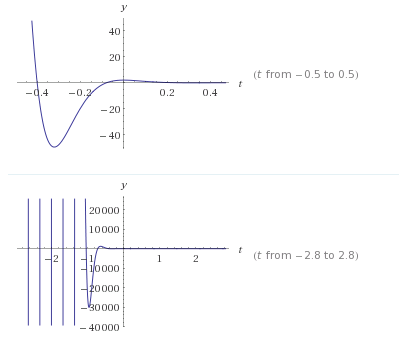
\includegraphics[scale=0.7]{prob1.png} \\
The quasi-frequency is \( \mu=4\sqrt{6} \) \\
The quasi-period is  \( T_d=\frac{\pi}{2\sqrt{6}} \)\\
The ratio is \( T_d/T=\frac{7}{2\sqrt{6}} \)

\end{homeworkProblem}

\begin{homeworkProblem}
\[
\begin{split}
	u''+2u=0\\
	u(0)=0 \\
	u'0)=2 \\
\end{split}
\]
We can get
\[
	u=Acos\sqrt{2}t+Bsin\sqrt{2}t
\]
Plug it in, we get
\[
	u=\sqrt{2}sin\sqrt{2}t
\]
We get the plot of the graph \\
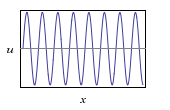
\includegraphics[scale=0.7]{prob2.png} \\
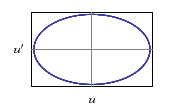
\includegraphics[scale=0.7]{prob3.png} \\


\end{homeworkProblem}

\begin{homeworkProblem}
(a)We can get 
\[
	u''+256u=0 
\]
So \[
	y=Acos(16t)+Bsin(16t)
\]
Comparing the equation and the 
\( mu''+ku=F_0coswt\)
We get \( w_0=16\)
So the equation becomes
\[
u=Acosw_0t+Bsinw_0t+\frac{F_0}{m(w^2_0-w^2)}coswt 
\]\\
\[ =Acos(16t)+Bsin(16t)+\frac{16}{247}cos(3t) \]
Plug it in with initial condition, we get
\[
 u=\frac{151}{1482}	cos16t+ \frac{16}{247} cos3t
\]
(b) Also we get the plot \\
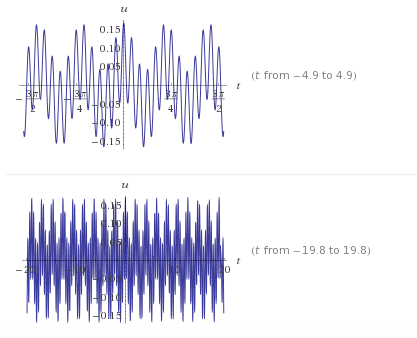
\includegraphics[scale=0.7]{prob4.png} \\
(c) 
The equation becomes
\[
	 mu''+ku=4sinwt
\]
And we can get
\[
u(t)=Acos(16t)+Bsin(16t)+U(t)
\]
Since \[ U(t)= \frac{32}{256-w^2}sinwt\]
\[ w=w_0=16 \]

\end{homeworkProblem}

\begin{homeworkProblem}
\textbf{Project}
\begin{verbatim}
function xp=F(t,x)
xp=zeros(2,1); % since output must be a column vector
e=-0.3;
xp(1)=x(2);
xp(2)=-e*x(1)^3-x(1);
\end{verbatim}

\textbf{Question 1} \\
We get the plot with e=0,0.2,0.4,0.6,0.8,1 \\
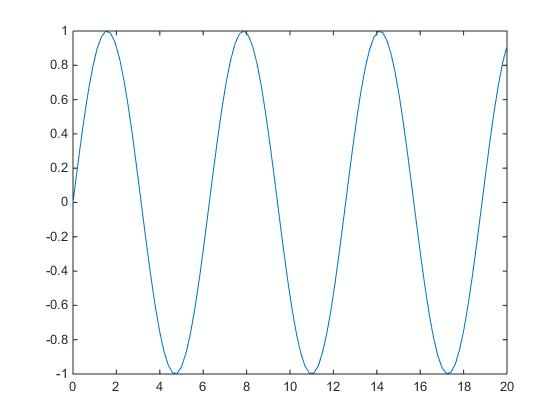
\includegraphics[scale=0.7]{10} \\
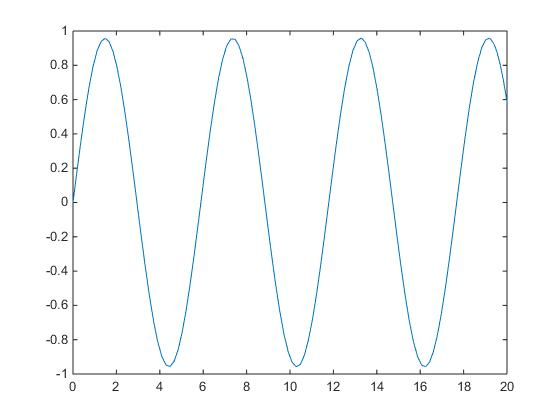
\includegraphics[scale=0.7]{12} \\
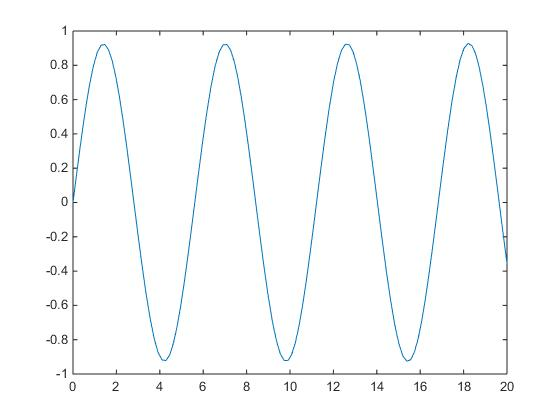
\includegraphics[scale=0.7]{14} \\
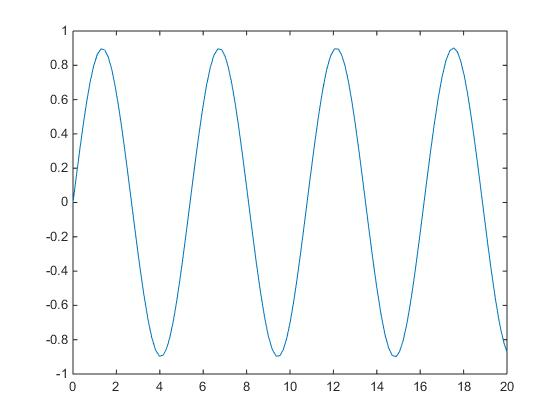
\includegraphics[scale=0.7]{16} \\
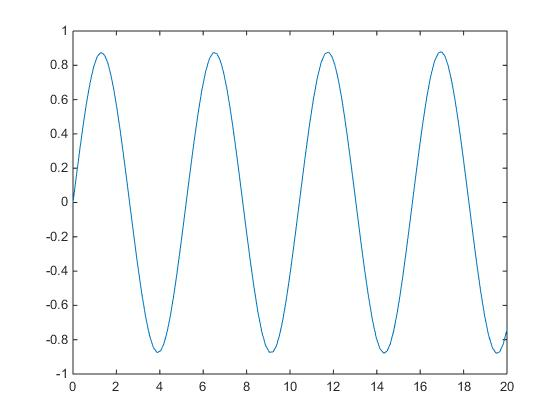
\includegraphics[scale=0.7]{18} \\
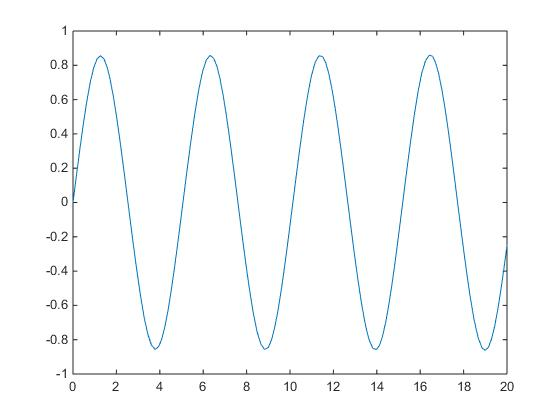
\includegraphics[scale=0.7]{110} \\
As I can see, as e goes toward infinity, the period is smaller. 
And the equilibrium equals to 3,2.8,2.6,2.4,2.2,2
So the \(u^+\) is smaller\\

\textbf{Question 2} \\
We get the plot with e=-0.1,-0.2,-0.3,-0.4 \\
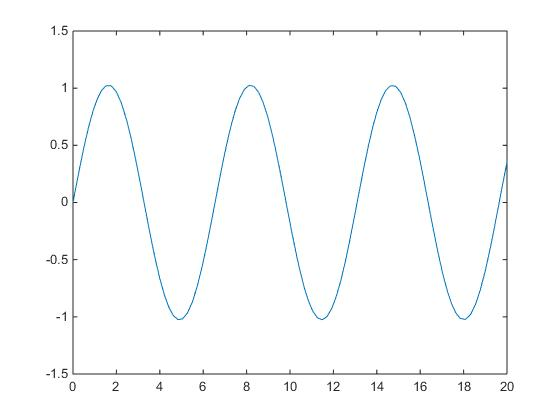
\includegraphics[scale=0.7]{201} \\
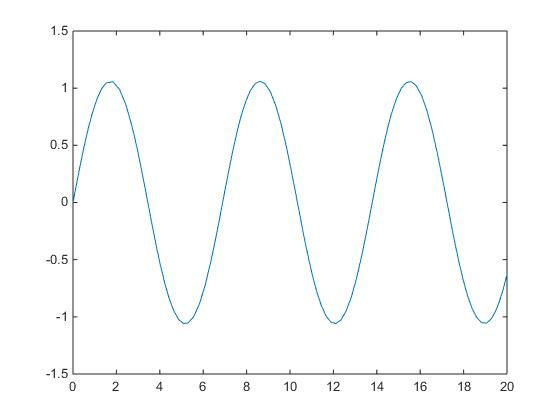
\includegraphics[scale=0.7]{202} \\
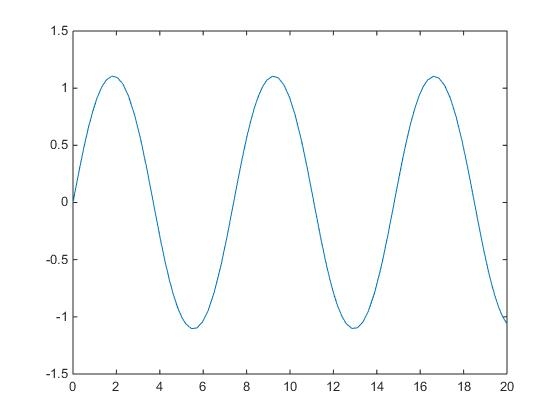
\includegraphics[scale=0.7]{203} \\
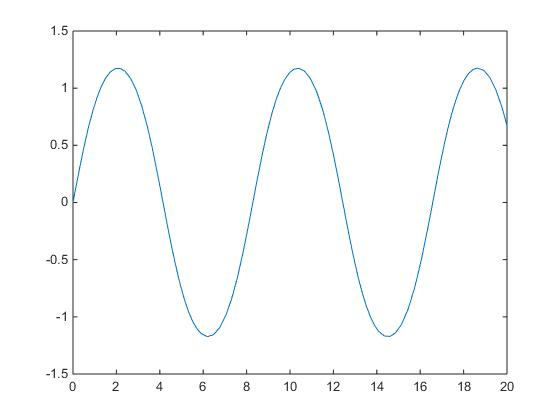
\includegraphics[scale=0.7]{204} \\
As I can see, as e goes toward negative infinity, the period is longer. \\
So the \(u^+\) is bigger\\
And the equilibrium equals to 3,3.2,3.4,3.6

\textbf{Question 3} \\
\begin{verbatim}
function xp=F(t,x)
xp=zeros(2,1); % since output must be a column vector
w=0.5;
xp(1)=x(2);
xp(2)=cos(w*t)-(1/5)*x(2)-x(1)-1/5*x(1)^3;
\end{verbatim}
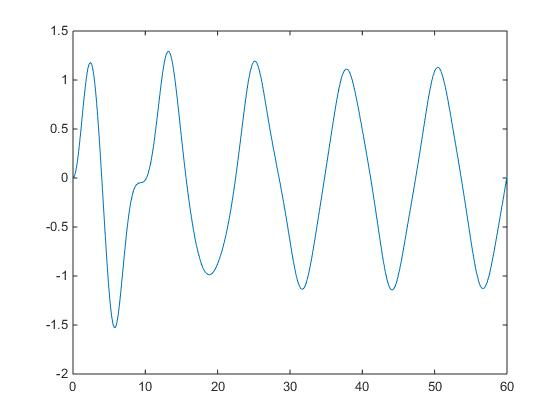
\includegraphics[scale=0.7]{305} \\
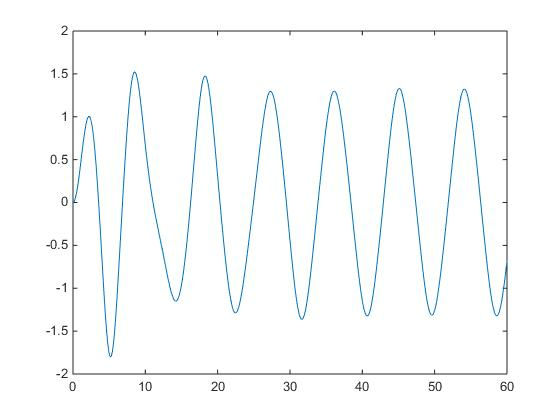
\includegraphics[scale=0.7]{307} \\
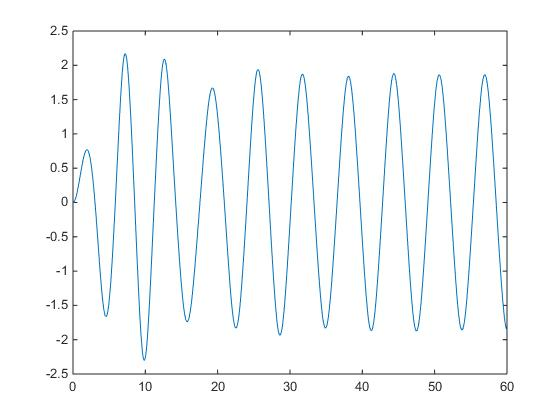
\includegraphics[scale=0.7]{310} \\
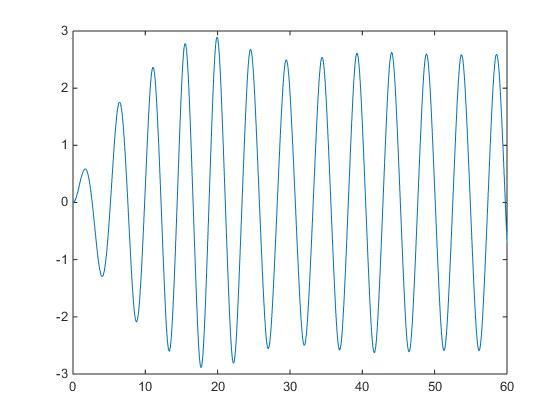
\includegraphics[scale=0.7]{313} \\
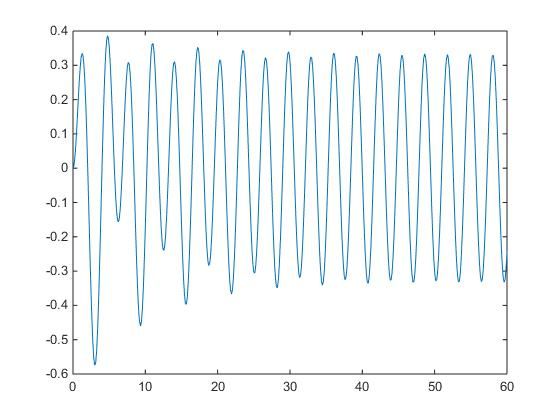
\includegraphics[scale=0.7]{320} \\

Based on my eyes, the w should be close to 1.4 which \(|u(t)|\) is largest.

\end{homeworkProblem}

\end{document}
